\documentclass[conference]{IEEEtran}
\IEEEoverridecommandlockouts
% The preceding line is only needed to identify funding in the first footnote. If that is unneeded, please comment it out.
\usepackage{cite}
\usepackage{amsmath,amssymb,amsfonts}
\usepackage{algorithmic}
\usepackage{graphicx}
\usepackage{textcomp}
\usepackage{xcolor}
\def\BibTeX{{\rm B\kern-.05em{\sc i\kern-.025em b}\kern-.08em
    T\kern-.1667em\lower.7ex\hbox{E}\kern-.125emX}}

\usepackage{listings}
\usepackage{color}

\definecolor{dkgreen}{rgb}{0,0.6,0}
\definecolor{gray}{rgb}{0.5,0.5,0.5}
\definecolor{mauve}{rgb}{0.58,0,0.82}

\lstdefinestyle{Python} {language=Python}

\lstset{frame=none,
	aboveskip=1mm,
	belowskip=1mm,
	showstringspaces=false,
	columns=flexible,
	basicstyle={\small\ttfamily},
	numbers=none,
	numberstyle=\tiny\color{gray},
	keywordstyle=\color{blue},
	commentstyle=\color{dkgreen},
	stringstyle=\color{mauve},
	breaklines=true,
	breakatwhitespace=true,
	tabsize=2
}

\begin{document}

\title{Work on simplifying and streamlining TPS}

\author{\IEEEauthorblockN{1\textsuperscript{st} Griffin Barrett}
\IEEEauthorblockA{
	\textit{Carleton University}\\
	Ottawa, Canada \\
	griffin-barrett@outlook.com}
}

\maketitle

\begin{IEEEkeywords}
Discrete event simulation, PDEVS
\end{IEEEkeywords}

\section{Introduction}

This report talks about work done in the area of simulation. Simulation is a powerful tool used to ask questions about the world that would be prohibitively expensive or impossible to ask directly. People have been simulating in one form or another for as long as we have had computers, and in fact it was a driving force behind some of the earliest digital computers that we know of. 

Today, the topics of simulations vary wildly from the very large to the very small to the very fast and everywhere in between. One such field is particle simulation. Many real world systems can be simplified down to particle simulation. Gases can be modeled as particles undergoing elastic collisions, and rope or other compliant structures can be modeled as chains or networks of connected particles. Having a good generally useful tool for simulating such systems would have wide practical uses.

\section{DEVS}

Discrete Event Simulation (DEVS) is a formal way of describing a discrete time simulation \cite{devs}. 

Under this formalism the system to be simulated is broken down into finitely many atomic models, that are the leaves on a tree of coupled models, culminating in the root of the tree, the top model. This is possible because of the ways in which the composition of coupled models exhibit closure. 

Models under DEVS each have an internal transition function, an external transition function, an output function, a time advance function, an internal state picked from a finite set of possible states, and a set of allowable inputs and outputs. This comes together to form a powerful enough and general enough framework to describe any possible discrete event system, including many other discrete event formalisms in their entirety. 

This system is clunky however, as it does not handle concurrent events very well. Parallel DEVS (PDEVS) is a formalism that expands upon DEVS just slightly, allowing it to handle these situations more naturally\cite{pdevs}. It adds one additional function, the confluence function, which acts as a tie breaker between the internal and external transition functions, and the ability to take more than one of each input and emit more than one of each output at the same time. It is the formalism of choice for this report.

\section{Existing Technique}

There is an existing implementation and formal description of a model for the stochastic event driven simulating a system of tethered particles under DEVS\cite{TPS-thesis}\cite{TPS-article}. The so called "Tethered Particle System" (TPS) implementation is designed to model biological systems, but extends to systems including airflow and fluid dynamics. This implementation works by having particles follow linear motion between events, and undergo discrete impulses from their environment to change their direction. These impulses come from two main sources, bumping into other particles (called blocking collisions) and reaching the limit of the extension on their connection to another particle (called tethering collisions). Between these two and simple Brownian and constant accelerations, many complex systems can be formed. 

The design of TPS aims to solve two main drawbacks of event based simulation of particle systems. The first of which is when a relatively light particle is trapped between two relatively massive particles and is made to act as a force carrier between them, taking dozens or even hundreds of collision events in an infinitesimally short amount of time. The second if when two tethered particles find themselves revolving at or near the limit of their range, with each tethered collision causing a minute change in direction again and again rather than a larger change less often.

These two issues are covered by a system of gluing particles together temporally to form groups that act as one larger particle, and instituting a minimum deflection angle to tethered collisions respectively.

\section{Contribution}

\subsection{Simplifying the internal mechanisum}

The existing TPS works well, but poses computational hurdles. In the existing implementation, volumes of interest overlap, necessitating duplication of calculations. This is easy to see because these volumes are described by spheres, which do not tile space neatly. This has the advantage of only needing to consider the contents of one volume at a time, but we can do better. With axis aligned boxes serving as volumes, there is no required overlap. This is not a complex thing to change, and even simplifies some of the code surrounding volume bounds checking. Each particle is in exactly one volume, and only needs to consider the volume that it is in and volumes no more than one step away in each axis. With some care and a sufficiently small volume size large gains can be found here.

Another shortcomings of the existing implementation is that collisions require allocating multiple one use objects, walking complex data structures, and deallocating a different set of objects, spread over an unbounded number of events. The new implementation proposed does away with most of this. No allocation is required. Only vectors and maps need to be traversed and even then only to a fixed depth. Collisions each create at most two events on their own. Some ground is lost in the case of three or more particles of vastly different masses colliding, but this is uncommon enough that as long as the new implementation is not appallingly slow the gains in the fast path of the simulation will make up for it.

\subsection{Simplifying the output format}

The existing simulator simply outputs the full state of each volume at each time step. This does guarantee not missing anything, but in the simple case of tracking the movement of the particles it is excessive. The total number of events grows faster than linear with the number of particles, leading to a log file size growth in excess of the number of particles squared multiplied by the total simulation time. Such a file quickly grows unwieldy and poses disk read speed related issues to parsers. The alternative is to look at the file containing only messages, but this too has shortcomings. Now velocity is left out of the logs, leaving only linear interpolation between start and end points. Such interpolation works, but because you need the end point before you can start, you effectively need the entire file loaded to use it. Parsers find the size of models that they can handle bounded by system memory or risk paying the price of paging to disk.

The proposed model instead stores both position and velocity in the messages that are passed, allowing a simple parser to access all that it needs to interpolate in a single pass of the file. The remaining constraints involve the total number of particles and the amount of information about each time that the parser saves, but these are things that all parsers will be limited by.


\section{Design Overview}

\subsection{Volume Model}

This atomic model contains the particles and has 3 jobs.

\begin{itemize}
	\item Apply incoming deltas
	\item Manage and apply deferred velocities at the right time
	\item Manage the movement of particles between volumes
\end{itemize}

It does this by calculating when each of its particles would leave and when each would have a deferred velocity to apply in its internal transition, and returning the minimum from its time advance, and mechanically applying deltas in its external transition. The existing implementation is rather aggressive with when it recalculates times, which is an area of further refinement, but the existing implementation works. 

\subsection{Blocking Collider Model}

This atomic acts on one or more volumes and has one job. It manages what happens when two particles undergo a blocking collision. That is to say, when they run into each other. By listening to and recording the latest announcement message from each volume, it has all the info that it needs to do this job.

In its external transition volumes that announce a change are flagged as dirty. After all messages have been read in, every particle in a dirty volume is checked against every particle in its own volume and every other volume that shares one or more corners with it. The soonest collision for each volume is cached to limit superfluous calculation. This could be extended to cache the soonest collision for each particle in the future, but that is not an issue of correctness.

In its internal transition, every cached collision has its deltas calculated and queued for the output function. This calculation is done in two parts. First an immediate delta velocity is calculated for each particle to bring their relative speed to a stop while conserving momentum. Second the deferred velocity required to send each particle away from the collision with their share of the kinetic energy again conserving momentum is calculated. These calculations also take into account a proportional amount of energy lost to damping effects specified by parameters, and also an extra separating force that grows proportionally to the number of collisions that each particle has been in since the last time its deferred velocity has been applied. This latter effect is to help pull apart clumps of particles that collide all at once creating thousands of events as they pass momentum around. The last consideration is that in the event of a second collision, the existing deferred velocity of each particle is applied at the time of the collision, but the timer is not reset. This prevents a potentially unbounded amount of energy from being stored in the deference leading to superluminal ejections.

\subsection{Tethered Collider Model}
This model works in much the same way as the Blocking Collider Model, except that instead of checking every pair of particles against the sum of their radii, they check a specified list of pairs of particles against an externally specified maximum distance.

The caching is done per pair, rather than per volume, and the collision code includes an extra term in the form of a minimum angle. This minimum angle prevents two tethered particles from orbiting one another too near their maximum distance again creating a potentially unbounded number of events.

\subsection{Rigid Collider Model}
This model has a list of faces. Each face is a point in a 1D simulation, a line segment in 2D, a triangle in 3D, and so on into higher spatial dimensions. These are the rigid bodies that this model manages the collisions of. They do not move, and represent parts of the environment.

Each face intersects one or more volumes, and each volume intersects with zero or more faces.

Much like the Tethered Collider Model and tethers, this model caches information about the next expected collision between a face and a particle for each face. Unlike the Blocking and Tethered Colliders, there are currently no extra terms about the collision. No energy is lost, no deferred velocity is calculated, particles simply bounce elastically off of the surface.

\subsection{Brownian Motion Model}
This model is the simplest to understand. Using the time Independent nature of the exponential distribution, it applies an impulse in a uniformly selected random direction with a normally distributed magnitude, to some particle selected at random. 

This is used to mimic the Brownian motion that would be seen if we had potentially far more particles in the system than we do, allowing for a computationally inexpensive way to scale a simulation up.

\section{Design Formal Definition}

\subsection{Data Types}
\begin{lstlisting}
Int  : Intager
UInt : Unsigned Int, an Int >= 0
Nat  : Natural Number, an Int > 0
Real : Some Real number, infinity, or negative infinity

PID : a Natural Number, uniquely identifying a particle
VID : a tuple of Integers, one per spatial dimension, describing a volume's position in the grid of all volumes

Vec : an N dimensional vector of Reals, where N is the number of spatial dimensions

Time : A Real, the type used to describe time

Particle : {
	last_updated : Time
	id           : PID
	species      : UInt
	mass         : Real
	radius       : Real
	position     : Vec, Where the particle was at t=last_updated
	velocity          : Vec
	deferred_velocity : Vec, what change of velocity has been deferred
	deferred_velocity_time       : Time, when will the deferred velocity be applied
	hits_while_velocity_deferred : UInt, how many collisions has this particle been in since the last time its deferred velocity has been applied
}, Particles in this simulation are represented by this type

Move_message : {
	destination : VID
	particle : Particle
}, Moving a particle is having it move from one volume to another, usually adjacent, volume, or a particle leaving the simulation area entirely.

Delta_message : {
	containing_volume : VID
	subject : PID
	delta_velocity : Vec
	delta_deferred_velocity : Vec
	deferred_velocity_time : Time
}, These are used to tell a volume that a change has happened to one of its contained particles. The velocities are added to the particles own and the soonest of particle's and the delta's deferred_velocity_time are used. The particle's hits_while_velocity_deferred is incremented.

Announcement_message : {
	id : VID
	particles_changed : List<PID>
	particles_moved   : List<PID>
	volume_contents_update : Map<PID, Particle>, the contents of the volume after these updates have been applied
}, Whenever a change happens within a volume, that volume announces that change using this message type

Face: A list of N Vecs where N is the number of spatial dimensions. This is a point in 1D, a line segment described by start and end point in 2D, a triangle in 3D, and so on. Used by the rigid collider

\end{lstlisting}

\subsection{Volume Model}
\begin{lstlisting}
state : {
	id        : VID, the location of this volume within the grid of all volumes
	position  : Vec, the position of one corner of the volume in space
	size      : Vec, the position of the oposite corner, measured from the first corner 
	particles : Map<PID, Particle>, all particles currently contained by this volume, as they are, indexed by their id
	
	pending_changes  : Set<PID> in particles, set of all particle ids whos particles have been changed since the last update
	pending_removals : Set<PID> not in particles, set of all particle ids whos particles have been moved out of this volume since the last update
	pending_moves    : Set<Move_message>
	
	next_internal_time : Time
	global_time        : Time
}

in_ports : {
	particle_entering : Move_message
	particle_delta    : Delta_message
}

out_ports {
	particle_leaving      : Move_message
	particle_announcement : Announcement_message
}
\end{lstlisting}

\begin{lstlisting}[style=Python]

def internal_transition(state):
	state.global_time += time_advance(state)
	
	state.pending_changes  = []
	state.pending_removals = []
	state.pending_moves    = []
	state.next_internal_time = inf;
	
	for pid, p in state.particles.items():
		move_out_time = particle_leave_time(p, state.position, state.size)
		
		if move_out_time <= state.global_time:
			state.pending_moves.append(
				Move_message(
					move_out_destination(p, state.position, state.size, state.position),
					p
				)
			)
			state.pending_removals.append(pid)
			state.particles.remove(pid)
			
		elif p.deferred_velocity_time <= state.global_time:
			state.particles [pid] = apply_deferred_velocity(p)
			state.pending_changes.append(pid)
		else:
			state.next_internal_time = min(state.next_internal_time, next_move_out_time, p.deferred_dv_time)
			
def external_transition(state, dt:Time, inputs):
	state.global_time += dt
	
	for move_msg in inputs.particle_entering:
		if move_msg.destination == state.id:
			state.particles [move_msg.particle.id] = move_msg.particle
			state.pending_updates.append( move_msg.particle.id)
	
	for delta_msg in inputs.particle_delta:
		if delta_msg.containing_volume = state.id:
			if delta_msg.subject in state.particles:
				state.particles [delta_msg.subject] = apply_delta(state.particles [delta_msg.subject], delta_msg)
				state.pending_changes.append( delta_msg.subject)
			else:
				#we got a delta for a particle that we do not have. It might be leaving at the same time, so we look for it in the pending moves
				for move_msg in state.pending_moves:
					if move_msg.particle.id == delta_msg.subject:
						move_msg.particle = apply_delta(move_msg.particle, delta_msg)
						#no need to announce it, the next volume will anounce it
						break
				else:
					warn("A delta has been lost")

def confluence_transition(state, dt:Time, inputs):
	internal_transition(state)
	external_transition(state, 0, inputs)

def output(state):
	outputs = output_bag(out_ports)
	
	for move_msg in state.pending_moves:
		outputs.particle_leaving.append(move_msg)
	
	if len(state.pending_changes) > 0 or len(state.pending_removals):
		outputs.particle_announcement.append(
			Announcement_message(
				state.id,
				state.pending_changes,
				state.pending_removals,
				const_copy(state.particles)
			)
		)
	
	return outputs

def time_advance(state):
	#if there is nothing waiting to be sent, we wait
	if len(state.pending_changes) == 0 and len(state.pending_removals) == 0 and len(state.pending_moves) == 0:
		return max(state.next_internal_time - state.global_time, 0)
	else:
		return 0

\end{lstlisting}

\subsection{Blocking Collider Model}
\begin{lstlisting}
state : {
	pending_deltas     : Set<Delta_message>
	
	volume_data        : Map<VID, Map<PID, Particle>>
	cache_data         : Map<VID, Tuple<PID, PID, VID, Time>>, id of particle in this volume that collides, id of particle it collides with, id of volume that the second particle is in, the time that they collide
	
	next_internal_time : Time
	global_time        : Time
}

in_ports : {
	particle_announcement : Announcement_message
}

out_ports {
	particle_delta    : Delta_message
}
\end{lstlisting}

\begin{lstlisting}[style=Python]
	
def internal_transition(state):
	state.global_time += time_advance(state)
	state.pending_deltas = []
	state.next_internal_time = inf
	
	for left_volume_id, (left_particle_id, right_particle_id, right_volume_id, collide_time) in state.cache_data.items():
		if collide_time <= state.global_time:
			left_delta, right_delta = blocking_collision(
				state.volume_data [left_volume_id] [left_particle_id],
				state.volume_data [right_volume_id] [right_particle_id],
				state.global_time,
				ENERGY_LOSSES:Real [0:1],
				STICK_TIME:Time,
				EXTRA_PUSH_FACTOR:Real [0:]
			)
			left_delta.containing_volume = left_volume_id
			right_delta.containing_volume = right_volume_id
			
			state.pending_deltas.append(left_delta)
			state.pending_deltas.append(right_delta)
			
			state.cache_data [left_volume_id] = (None, None, None, inf)
	
def external_transition(state, dt:Time, inputs):
	state.global_time += dt
	dirty_volume_ids = []:Set<VID>
	
	for a_msg in inputs.particle_announcement:
		dirty_volume_ids.append(a_msg.id)
		state.cache_data [a_msg.id] = (None, None, None, inf) #we do not know this volume's next collision anymore
		state.volume_data [a_msg.id] = a_msg.volume_contents_update
		
	for left_volume_id in dirty_volume_ids:
		for right_volume_id in set_of_volume_ids_within_one_step_of( left_volume_id):
			for left_particle_id in state.volume_data [left_volume_id]:
				for right_particle_id in state.volume_data [right_volume_id]:
					left_particle = state.volume_data [left_volume_id] [left_particle_id]
					right_particle = state.volume_data [right_volume_id] [right_particle_id]
					collide_time = blocking_collision_time( left_particle, right_particle):
					if collide_time < inf and collide_time >= state.global_time:
						state.next_internal_time = min(state.next_internal_time, collide_time)
						#cach_data [4] is the time of the next collision
						if left_particle_id < right_particle_id and collide_time < state.cache_data [left_volume_id] [3]:
							state.cache_data [left_volume_id] = (left_particle_id, right_particle_id, right_volume_id, collide_time)
						elif collide_time < state.cache_data [right_volume_id] [3]:
							state.cache_data [right_volume_id] = (right_particle_id, left_particle_id, left_volume_id, collide_time)
	
def confluence_transition(state, dt:Time, inputs):
	internal_transition(state)
	external_transition(state, 0, inputs)
	
def output(state):
	outputs = output_bag(out_ports)
	for delta in state.pending_deltas:
		outputs.particle_delta.append(delta)
	return outputs
	
def time_advance(state):
	if len(state.pending_deltas) > 0:
		return 0
	else:
		return max(state.next_internal_time - state.global_time , 0)
	
\end{lstlisting}

\subsection{Tethered Collider Model}
\begin{lstlisting}
state : {
	tethers   : List<Tuple<PID, PID, Real>>, the ID of two particles and the maximum distance between them
	particles : Map<PID, Set<UInt>>, the particle ID to the set of tethers it is a part of
	cache     : Map<UInt, Tuple<VID, VID, Time>>, The index into the list of tethers, and the two volumes that the particle can be found in, and the time of their next colission

	volume_data        : Map<VID, Map<PID, Particle>>
	
	pending_deltas     : Set<Delta_message>
	
	next_internal_time : Time
	global_time        : Time
}

in_ports : {
	particle_announcement : Announcement_message
}

out_ports {
	particle_delta : Delta_message
}

\end{lstlisting}
\begin{lstlisting}[style=Python]
	
def internal_transition(state):
	state.global_time += time_advance(state)
	state.pending_deltas = []
	state.next_internal_time = inf
	
	for t_id, (left_volume_id, right_volume_id, collide_time) in state.cache.items():
		if collide_time <= state.global_time:
			left_pid, right_pid, radius = state.tethers[t_id]
			left_delta, right_delta = tethering_collision( state.state.volume_data [left_volume_id][left_pid], state.state.volume_data [right_volume_id][right_pid], radius, ENERGY_LOSSES:Real [0:1],
STICK_TIME:Time,
EXTRA_PUSH_FACTOR:Real [0:], MINIMUM_ANGLE:Real [0:PI/2])
			left_delta.left_delta.containing_volume = left_volume_id
			right_delta.right_delta.containing_volume = right_volume_id
			state.pending_deltas.append(left_delta)
			state.pending_deltas.append(right_delta)
			
			state.cache[t_id][2] = inf
			
def external_transition(state, dt:Time, inputs):
	state.global_time += dt
	
	Set<UInt> dirty_tethers = []
	
	for a_msg in inputs.particle_announcement:
		state.volume_data[a_msg.id] = a_msg.volume_contents_update
		for pid in a_msg.particles_changed:
			if pid in state.particles:
				for t_id in state.particles[pid]:
					dirty_tethers.append(t_id)
					if state.tethers[t_id][0] == pid:
						state.cache[t_id][0] = a_msg.id
					if state.tethers[t_id][1] == pid:
						state.cache[t_id][1] = a_msg.id
	for t_id in dirty_tethers:
		#cache[2] is the time of the next tethered collision
		state.cache[t_id][2] = tethered_collision_time( 
			state.volume_data[state.cache[t_id][0]] [state.tethers[t_id][0]],
			state.volume_data[state.cache[t_id][1]] [state.tethers[t_id][1]],
			state.tethers[t_id][2],
		)
		state.next_internal_time = min(state.next_internal_time, state.cache[t_id][2])
	
def confluence_transition(state, dt:Time, inputs):
	internal_transition(state)
	external_transition(state, 0, inputs)
	
def output(state):
	outputs = output_bag(out_ports)
	for delta in state.pending_deltas:
		outputs.particle_delta.append(delta)
	return outputs
	
def time_advance(state):
	if len(state.pending_deltas) > 0:
		return 0
	else:
		return max(state.next_internal_time - state.global_time, 0)
	
\end{lstlisting}

\subsection{Rigid Collider Model}
\begin{lstlisting}
state : {
	faces             : List<Face>, every rigid  body face that this model maintains
	f_v_intersections  : Map<UInt, Set<VID>>, for each face, every volume that it intersects with
	v_f_intersections  : Map<VID, Set<UInt>>, for each volume, every face that it intersects with
	
	cache              : Map<UInt, Tuple<VID, PID, Time>>, for each face, the next volume and particle to collide with it, and the time that they will collide
	
	volume_data        : Map<VID, Map<PID, Particle>>
	
	pending_deltas     : Set<Delta_message>
	
	next_internal_time : Time
	global_time        : Time
}

in_ports : {
	particle_announcement : Announcement_message
}

out_ports {
	particle_delta : Delta_message
}
\end{lstlisting}
\begin{lstlisting}[style=Python]
	
def internal_transition(state):
	state.global_time += time_advance(state)
	state.pending_deltas = []
	state.next_internal_time = inf
	
	for f_id, (vid, pid, collision_time) in state.cache.items():
		if collision_time <= state.global_time:
			delta = rigid_collision(state.faces[f_id], state.volume_data[vid][pid], collision_time)
			delta.containing_volume = vid
			state.pending_deltas.append(delta)
			state.cache[f_id] = (None, None, inf)
	
	
def external_transition(state, dt:Time, inputs):
	state.global_time += dt
	
	Set<UInt> dirty_faces = []
	
	for a_msg in inputs.particle_announcement:
		state.volume_data[a_msg.id] = a_msg.volume_contents_update
		for f_id in state.v_f_intersections[a_msg.id]:
			dirty_faces.append(f_id)
	
	for f_id in dirty_faces:
		face = state.faces[f_id]
		state.cache[f_id] = (None, None, inf)
		for vid in state.f_v_intersections[f_id]:
			for pid, particle in state.volume_data[vid].items():
				collision_time = next_rigid_collission(patricle, face, state.global_time)
				if collision_time <= state.cache[f_id][2] and collision_time >= state.global_time:
					state.cache[f_id] = (vid, pid, collision_time)
					state.next_internal_time = min(state.next_internal_time, collision_time)
	
def confluence_transition(state, dt:Time, inputs):
	internal_transition(state)
	external_transition(state, 0, inputs)
	
def output(state):
	outputs = output_bag(out_ports)
	for delta in state.pending_deltas:
		outputs.particle_delta.append(delta)
	return outputs
	
def time_advance(state):
	if len(state.pending_deltas) > 0:
		return 0
	else:
		return max(state.next_internal_time - state.global_time, 0)
	
\end{lstlisting}

\subsection{Brownian Motion Model}
\begin{lstlisting}
	state : {
		volume_data        : Map<VID, Map<PID, Particle>>
		total_particles    : UInt
		next_internal_time : Time
	}
	
	in_ports : {
		particle_announcement : Announcement_message
	}
	
	out_ports {
		particle_delta : Delta_message
	}
\end{lstlisting}
\begin{lstlisting}[style=Python]
	
def internal_transition(state):
	state.next_internal_time = exponentially_distributed_random(BETA, state.total_particles)
	
def external_transition(state, dt:Time, inputs):
	state.next_internal_time = max(state.next_internal_time - dt, 0)
	
	for a_msg in inputs.particle_announcement:
		state.volume_data[a_msg.id] = a_msg.volume_contents_update
		
def confluence_transition(state, dt:Time, inputs):
	internal_transition(state)
	external_transition(state, 0, inputs)
	
def output(state):
	outputs = output_bag(out_ports)
	
	impulse = brownian_impulse()
	
	vid, particle = uniformally_randomly_selected_volume_and_particle(state.volume_data)
	
	delta = apply_impulse_to_particle(particle, impulse)
	delta.id = vid
	
	outputs.particle_delta.append(delta)
	
	return outputs
	
def time_advance(state):
	return state.next_internal_time
	
\end{lstlisting}

\section{Practical Implementation So Far}

Work on a C++ implementation of the above model is ongoing. So far, Volume and Blocking Collision models have been completed. Below are some example outputs.

\begin{figure}[htbp]
	\centerline{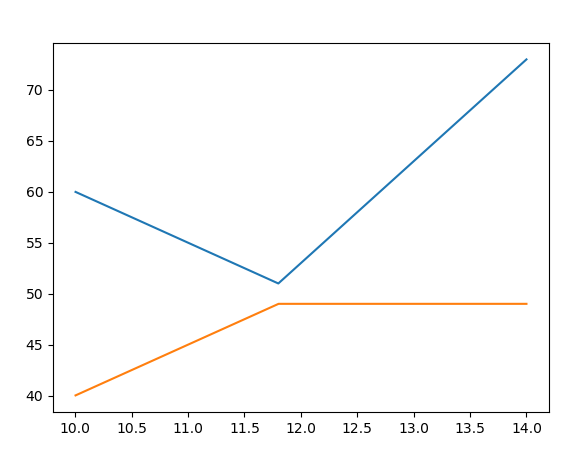
\includegraphics[width=0.7\columnwidth]{./figs/2p.png}}
	\caption{2 particles colliding in 2D. X and Y scale in meters. Each particle starts on the left and has a radius of 1m. The upper particle has a mass of 1kg, the lower 3kg}
	\label{2p}
\end{figure}

Figure \ref{2p} shows two particles colliding with one another in 2D space. In this example of two particles interacting, we are observing momentum being conserved. They each start moving at 10m/s towards each other and 2m/s to the right. The lower body has three times the mass of the upper body. After the impact, the lower particle has given all of its vertical momentum to the upper particle, and their horizontal moment is unchanged. This is to be expected.

\begin{figure}[htbp]
	\centerline{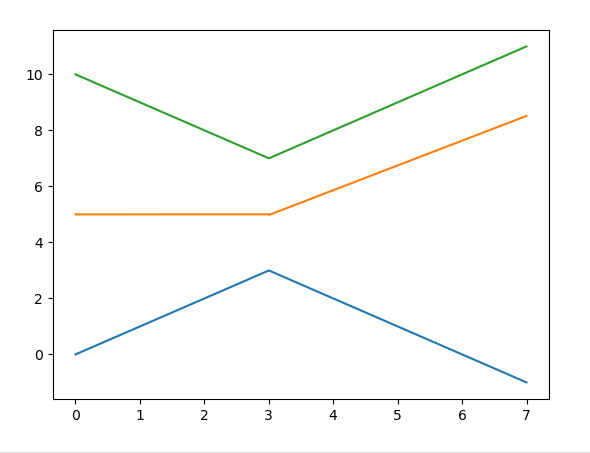
\includegraphics[width=0.7\columnwidth]{./figs/3p.png}}
	\caption{3 particles colliding in 2D. X and Y scale in meters. Each particle starts on the left and has a radius of 1m. The middle particle has a mass of 1g, while the upper and lower particle both have a mass of 1,000kg}
	\label{3p}
\end{figure}

Figure \ref{3p} is a stress test. The upper and lower particles each have a mass one million times the mass of the middle particle. The two outer bodies never directly interact with one another, and instead they need to pass all of their momentum through the inner body. In a naive implementation, 10 000 collisions are required to complete the exchange, each of which potentially pico-seconds apart. This diminutive time step all but disqualifies constant time simulations, and the colossal number of time advances makes such a situation computationally challenging for a naive discrete time simulator. This model's technique of having a short "stuck time" on impacts allows the collisions to walk forward until the point at which all three particles are touching, then the remaining momentum is exchanged in a series of time-advance-zero events, which modern event driven simulators excel at optimizing \cite{time-advance-0}. The addition of dumping deferred velocity and applying an extra pushing force allows this model to finish in only 2 000 events, an 80\% improvement on raw count alone, over and above the time saved by any optimizations provided by the runner.

In the TPS implementation in the literature \cite{TPS-thesis}\cite{TPS-article}, this would potentially have taken only one large event. This would look like the work done here is a severe degradation, but remember, the calculations preformed by this model are far faster in the more common cases while not being too terrible in exceptional cases like this one. 


\section{Future Work}

Future work in this area includes completing the implementation, refining the caching strategies used, expending the kinds of effects that can be described by the provided models, and expanding the tooling around the model.

In the current state of the project, only simple movement and blocking collisions are implemented. Far more are formally described, but more work is needed to make it usable.

Caching strategy selection is a historically hard problem, and this project is no exception. More work needs to be done in implementing varied strategies and testing them under different conditions.

While the above described models cover a wide range of situations, there are situations that they do not naturally extend to. Examples include a region of constant acceleration under gravity, the acceleration of charged particles in an electric field under the right hand rule, and the creation and destruction of particles. These situations are within reach of this model, but formal descriptions are not yet available.

The tooling surrounding these models is lacking. Output can be charted as in figures \ref{2p} and \ref{3p}, and the code to do so is extendable, but such output is limited to 1D and 2D experiments. On the other end of the pipeline, the initial conditions are compiled in to the program, making fast iteration on experiment design an exercise in waiting on gcc. This too can be fixed. Aside from the number of spatial dimensions and the level of numerical precision, everything else could be specified in an external configuration file.

These four topics represent obvious areas for future improvements.

\begin{thebibliography}{00}
	
	\bibitem{TPS-thesis} R. Goldstein, ``DEVS-Based Dynamic Simulation of Deformable Biological Structures,''  M.S. thesis, Carleton University, Ottawa Canada, Sept. 2009, [Online] Available: http://cell-devs.sce.carleton.ca/publications/2009/Gol09/
	
	\bibitem{TPS-article} R. Goldstein and G. Wainer, ``Impulse-Based Dynamic Simulation of Deformable Biological Structures'' Transactions on Computational Systems Biology, Springer-Verlag, 2011, pp. 39-60, Available: http://cell-devs.sce.carleton.ca/publications/2011/GW11
	
	\bibitem{devs} Radiya, Ashvin, and Robert Sargent. ``A Logic-Based Foundation of Discrete Event Modeling and Simulation.'' ACM Transactions on Modeling and Computer Simulation, vol. 4, no. 1, ACM, 1994, pp. 3–51, doi:10.1145/174619.174620.
	
	\bibitem{pdevs}A. C. H. Chow and B. P. Zeigler, ``Parallel DEVS: a parallel, hierarchical, modular modeling formalism,'' Proceedings of Winter Simulation Conference, 1994, pp. 716-722, doi: 10.1109/WSC.1994.717419.
	
	\bibitem{time-advance-0} C. R. Martin, G. G. Trabes and G. A. Wainer, ``A New Simulation Algorithm for PDEVS Models with Time Advance Zero,'' 2020 Winter Simulation Conference (WSC), 2020, pp. 2208-2220, doi: 10.1109/WSC48552.2020.9384028.
	
\end{thebibliography}
\end{document}
